\documentclass[preprint,12pt]{elsarticle}

\usepackage{amsmath}
\usepackage{booktabs}
\usepackage{graphicx}
\usepackage{hyperref}
\usepackage{tabularx}
\usepackage{xurl}
\hypersetup{hidelinks}

\journal{SoftwareX}
\graphicspath{{figures/}}
\emergencystretch=1em

\begin{document}

\begin{frontmatter}

\title{HomiCSx: An end-to-end FEniCSx framework for finite-element computational homogenization}

\author{Amir Reza Tahouni\corref{cor1}}
\ead{tahouniamirreza@gmail.com}
\address{Independent researcher, Tehran, Iran}
\cortext[cor1]{Corresponding author}

\begin{abstract}
HomiCSx is an open-source FEniCSx framework that connects particulate geometry,
periodic-conforming Gmsh meshing, material assignment, linear and finite-strain
periodic homogenization, hooks, and essential outputs in one reproducible
pipeline. Its supported core includes two- and three-dimensional cells,
multiphase linear elasticity, user-defined hyperelastic energies with a
built-in Neo-Hookean model, and generalized-Maxwell viscoelasticity.
Verification combines analytical tests, constitutive checks, mesh refinement,
regression gates, and cross-solver comparisons using independently constructed
Abaqus models and conventional
macroscopic quantities. Canonical linear discrepancies remain below 0.55\%, and
tested heterogeneous viscoelastic histories remain within 1.36\%. HomiCSx
targets inspectable, customizable computational-homogenization studies with an
explicitly bounded support and maintenance scope.
\end{abstract}

\begin{keyword}
computational homogenization \sep finite element method \sep FEniCSx \sep
representative volume element \sep composite materials \sep viscoelasticity
\end{keyword}

\end{frontmatter}

\begin{table}[htbp]
\centering
\small
\begin{tabularx}{\linewidth}{@{}p{0.06\linewidth}p{0.38\linewidth}X@{}}
\toprule
Nr & Code metadata description & Metadata \\
\midrule
C1 & Current code version & v1.0.1 \\
C2 & Permanent link to code/repository used for this code version &
\href{https://github.com/AmirTahouni/HomiCSx/tree/v1.0.1}{GitHub v1.0.1 tag} \\
C3 & Legal code license & MIT \\
C4 & Code versioning system used & Git \\
C5 & Software code languages, tools and services used & Python, NumPy, UFL,
DOLFINx, PETSc/petsc4py, Basix, Gmsh API, MPI \\
C6 & Compilation requirements, operating environments and dependencies &
Conda; Python 3.10; DOLFINx 0.9.0; dolfinx\_mpc 0.9.0; Linux or WSL2 \\
C7 & Link to developer documentation/manual &
\url{https://homicsx.readthedocs.io/en/latest/} \\
C8 & Support email for questions &
\href{mailto:tahouniamirreza@gmail.com}{tahouniamirreza@gmail.com} \\
\bottomrule
\end{tabularx}
\caption{SoftwareX code metadata for HomiCSx.}
\label{tab:metadata}
\end{table}

\section{Motivation and significance}

First-order computational homogenization obtains macroscopic constitutive
response from microscopic boundary-value problems under scale separation
\cite{geers2003,saeb2016}. Its finite-element realization requires a chain of
choices that are often implemented in separate research scripts: constructing
a representative cell, preserving periodic geometry, producing compatible
opposite-boundary meshes, assigning phases, enforcing periodic constraints,
solving multiple macroscopic load cases, and reducing microscopic fields to
macroscopic quantities. This fragmentation makes it difficult to adapt a
workflow without also weakening its traceability.

HomiCSx provides these steps through a common set of Python data objects and
drivers built on DOLFINx and UFL \cite{dolfinx2025,ufl2014}, with geometry and
meshing provided by Gmsh \cite{gmsh2009}. Its main contribution is not a new
homogenization theory. It is an extensible end-to-end implementation in which
the geometry, discretization, constitutive response, macroscopic loading,
nonlinear solution, and result extraction remain explicit and replaceable.
This is useful for studies that require systematic microstructure generation
or research-specific operations during a nonlinear homogenization history.

The software supports linear and finite-strain problems in two and three
dimensions. Research-specific behavior can be introduced through custom
material implementations, callable load cases, and typed hooks invoked at
documented points in the nonlinear driver. The package therefore occupies a
middle ground between one-off finite-element scripts and closed workflows that
offer limited intervention in the solution sequence.

\subsection{Positioning relative to related software}

HomiCSx complements rather than replaces broader research-software ecosystems.
MicroStructPy emphasizes statistical microstructure generation and mesh export
\cite{microstructpy2020}, while HomiCSx couples a narrower particulate generator
directly to periodic mechanical solves. DAMASK provides mature grid and mesh
solvers for crystal-plasticity and multiphysics homogenization
\cite{damask2020}; HomiCSx instead targets compact, script-level customization
of particulate FEniCSx workflows. MOOSE is a general parallel finite-element
and multiphysics framework with periodic-boundary infrastructure
\cite{moose2020}, whereas HomiCSx packages domain-specific geometry, matching
periodic meshing, constitutive hooks, homogenization loads, and macro outputs
behind Python objects. HomiCSx does not claim their breadth, parallel
scalability, or adoption. Its narrower contribution is an inspectable serial
path joining these stages for linear, hyperelastic, and generalized-Maxwell
RVE studies. Closer code-level comparators include micmacsfenics, which targets
FEniCS/FEniCSx FE$^2$ and periodic or minimally constrained multiscale
problems, and FEniCS\_homogenization, a collection of legacy-FEniCS linear
elasticity scripts \cite{micmacsfenics,fenicshomogenization}. They demonstrate
that FEniCS-based homogenization implementations exist; the comparison set was
therefore selected to cover both these direct implementations and broader
geometry, constitutive, and multiphysics ecosystems. HomiCSx's claimed
distinction is the documented integration of particulate generation,
periodic-conforming meshing, finite-strain/history-dependent workflows, hooks,
and conventional validation rather than a claim to originate FEniCS
homogenization.

\section{Software description}

\subsection{Architecture and workflow}

The workflow has five cooperating layers. The geometry layer creates seeded,
periodic particulate cells or accepts explicitly constructed inclusions. The
mesh layer builds the corresponding OpenCASCADE model, assigns physical tags,
and generates triangular, tetrahedral, or supported two-dimensional
all-quadrilateral meshes. Opposite boundaries are meshed
with translated Gmsh periodic constraints so their nodes match. The material
layer maps phase identifiers to constitutive objects. The finite-element layer
constructs linear or nonlinear periodic fluctuation problems and applies
multipoint constraints. Finally, homogenization drivers execute standard or
user-defined macroscopic load cases and return macroscopic histories and
optional fields.

The core geometry types include circular and elliptical inclusions in 2D and
spherical and ellipsoidal inclusions in 3D, with monodisperse or polydisperse
sampling and clearance control. Periodic images retain source identity so that
boundary-split particles are represented consistently. Geometry generation is
seedable for reproducibility. Explicitly prescribed ellipses and ellipsoids may
be rotated; random nonspherical packing remains axis-aligned. The
publication-supported discretization path uses triangles, tetrahedra, or the
tested two-dimensional all-quadrilateral option for linear and
history-independent hyperelastic workflows. Generalized-Maxwell state updates
require simplex cells. General three-dimensional hexahedral meshing is outside
the current support boundary.

\subsection{Homogenization formulation}

For linear elasticity, the microscopic displacement is decomposed into a
macroscopic affine field and a periodic fluctuation. Elementary macroscopic
strain probes recover the effective stiffness from volume-averaged stress. In
finite strain, the deformation gradient is decomposed as
\begin{equation}
  \mathbf{F}(\mathbf{X}) = \bar{\mathbf{F}} +
  \nabla\widetilde{\mathbf{u}}(\mathbf{X}),
\end{equation}
where the fluctuation is periodic on opposite cell boundaries. The nonlinear
driver solves incremental equilibrium with adaptive stepping and records
volume-averaged first Piola--Kirchhoff stress, energy, deformation Jacobian,
and optional finite-difference tangent information for hyperelastic and
generalized-Maxwell materials.

Hyperelastic material objects provide a UFL strain-energy density and matching
numerical post-processing methods. Compressible Neo-Hookean elasticity is the
built-in, externally compared implementation; custom laws remain the user's
validation responsibility. For generalized-Maxwell branch $i$, let
$\mathbf{C}=\mathbf{F}^{T}\mathbf{F}$ and let $\mathbf{C}_{v,i}$ be its viscous
metric. HomiCSx implements
\begin{equation}
\Psi_i=\frac{\mu_i}{2}\left[\operatorname{tr}(\mathbf{C}\mathbf{C}_{v,i}^{-1})
-d-\ln\det(\mathbf{C}\mathbf{C}_{v,i}^{-1})\right],
\end{equation}
with nonequilibrium stress
$\mathbf{P}_i=\mu_i\mathbf{F}(\mathbf{C}_{v,i}^{-1}-\mathbf{C}^{-1})$.
Starting from $\mathbf{C}_{v,i}^{0}=\mathbf{I}$, a converged increment updates
\begin{equation}
\mathbf{C}_{v,i}^{n+1}=\alpha_i\mathbf{C}_{v,i}^{n}
+(1-\alpha_i)\mathbf{C}^{n+1},\qquad
\alpha_i=\exp(-\Delta t/\tau_i).
\end{equation}
The metrics are DG0 cellwise coefficients, consistent with the current
cellwise deformation-gradient evaluation. Previous converged metrics remain
fixed while global equilibrium is solved; trial state is committed only after
convergence. The total stress is the equilibrium hyperelastic stress plus all
branch stresses, so nonequilibrium stress enters the weak residual and its
Newton Jacobian is obtained by automatic differentiation. Objectivity follows
from dependence on $\mathbf{C}$ and an objective internal metric. Positive
branch moduli and relaxation times are required. In the Abaqus comparison,
$\tau_i$ is unchanged and the shear Prony ratio is
$g_i=\mu_i/(\mu_{\infty}+\sum_j\mu_j)$ with zero bulk Prony ratio.

The reported generalized-Maxwell macroscopic tangent is step-consistent. Each
positive and negative macro-deformation perturbation restarts from the same
previous converged viscous metrics, advances over the actual current time
increment, and resolves periodic equilibrium. Central differences form the
tangent columns, after which HomiCSx restores the unperturbed fluctuation field
and committed metrics. A one-sided difference is used if only one perturbation
converges.

\subsection{Customization and outputs}

Users can define macroscopic deformation histories as Python callables and can
derive new nonlinear material classes through the public material interface.
Hooks provide controlled access before and after documented stages of the
homogenization loop. They have explicit ordering and state scopes and can be
used to collect fields, compute application-specific metrics, or implement
additional workflow logic. Core outputs include effective stiffness, macro
stress/strain/energy histories and Jacobian histories. Finite-difference
tangents cover hyperelastic and generalized-Maxwell materials. Reconstructed
stress/energy XDMF fields remain limited to history-independent materials;
state-aware viscoelastic fields are available to hooks.
Figure~\ref{fig:architecture} summarizes this division between the supported
pipeline and its documented extension points.

\begin{figure}[htbp]
  \centering
  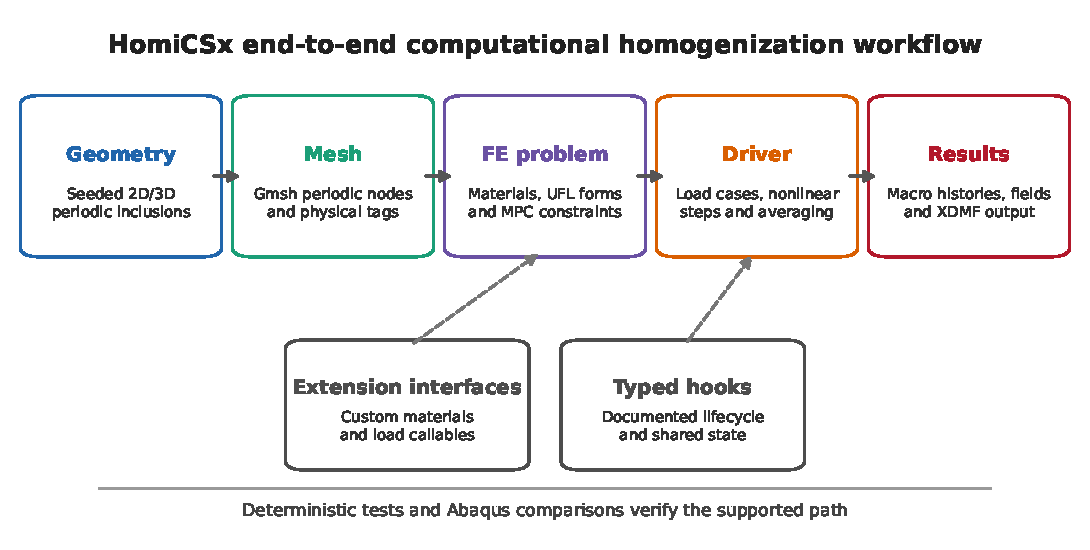
\includegraphics[width=\linewidth]{architecture_workflow.pdf}
  \caption{HomiCSx architecture and data flow. The supported workflow proceeds
  from geometry through periodic meshing, finite-element construction,
  homogenization, and result extraction. Custom materials, load callables, and
  typed hooks expose documented extension points.}
  \label{fig:architecture}
\end{figure}

\section{Illustrative examples}

The documentation demonstrates geometry generation, 2D and 3D linear solves,
hyperelasticity, generalized-Maxwell response, and typed hooks. A single
repository-level examples directory provides compact deterministic geometry,
2D/3D linear, hyperelastic, and heterogeneous viscoelastic
workflows; all five serial scripts are executed by the test suite. The linear script creates a
fixed geometry, generates a periodic-conforming mesh, assigns phase materials,
and passes these objects to the linear driver. The viscoelastic script exercises
nonlinear equilibrium, state evolution, and a typed macro-stress hook. The same
separation of concerns allows a geometry or material implementation to be
changed without replacing the full pipeline. Figure~\ref{fig:meshes}
illustrates the matching periodic boundary patterns produced by the meshing
stage, while Figure~\ref{fig:fields} shows representative field output opened
in ParaView.

\begin{figure}[htbp]
  \centering
  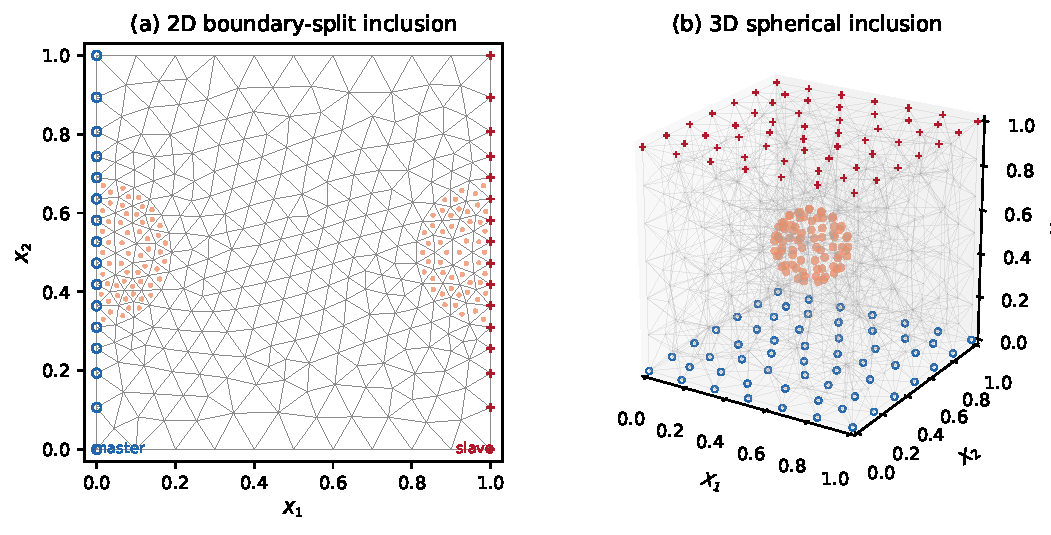
\includegraphics[width=\linewidth]{periodic_meshes.pdf}
  \caption{Representative periodic-conforming HomiCSx meshes. The 2D cell
  contains one physical circle split across the left/right boundary; the 3D
  cell contains a centered sphere. Blue circles mark master-face nodes and red
  crosses mark matching slave-face patterns.}
  \label{fig:meshes}
\end{figure}

\begin{figure}[htbp]
  \centering
  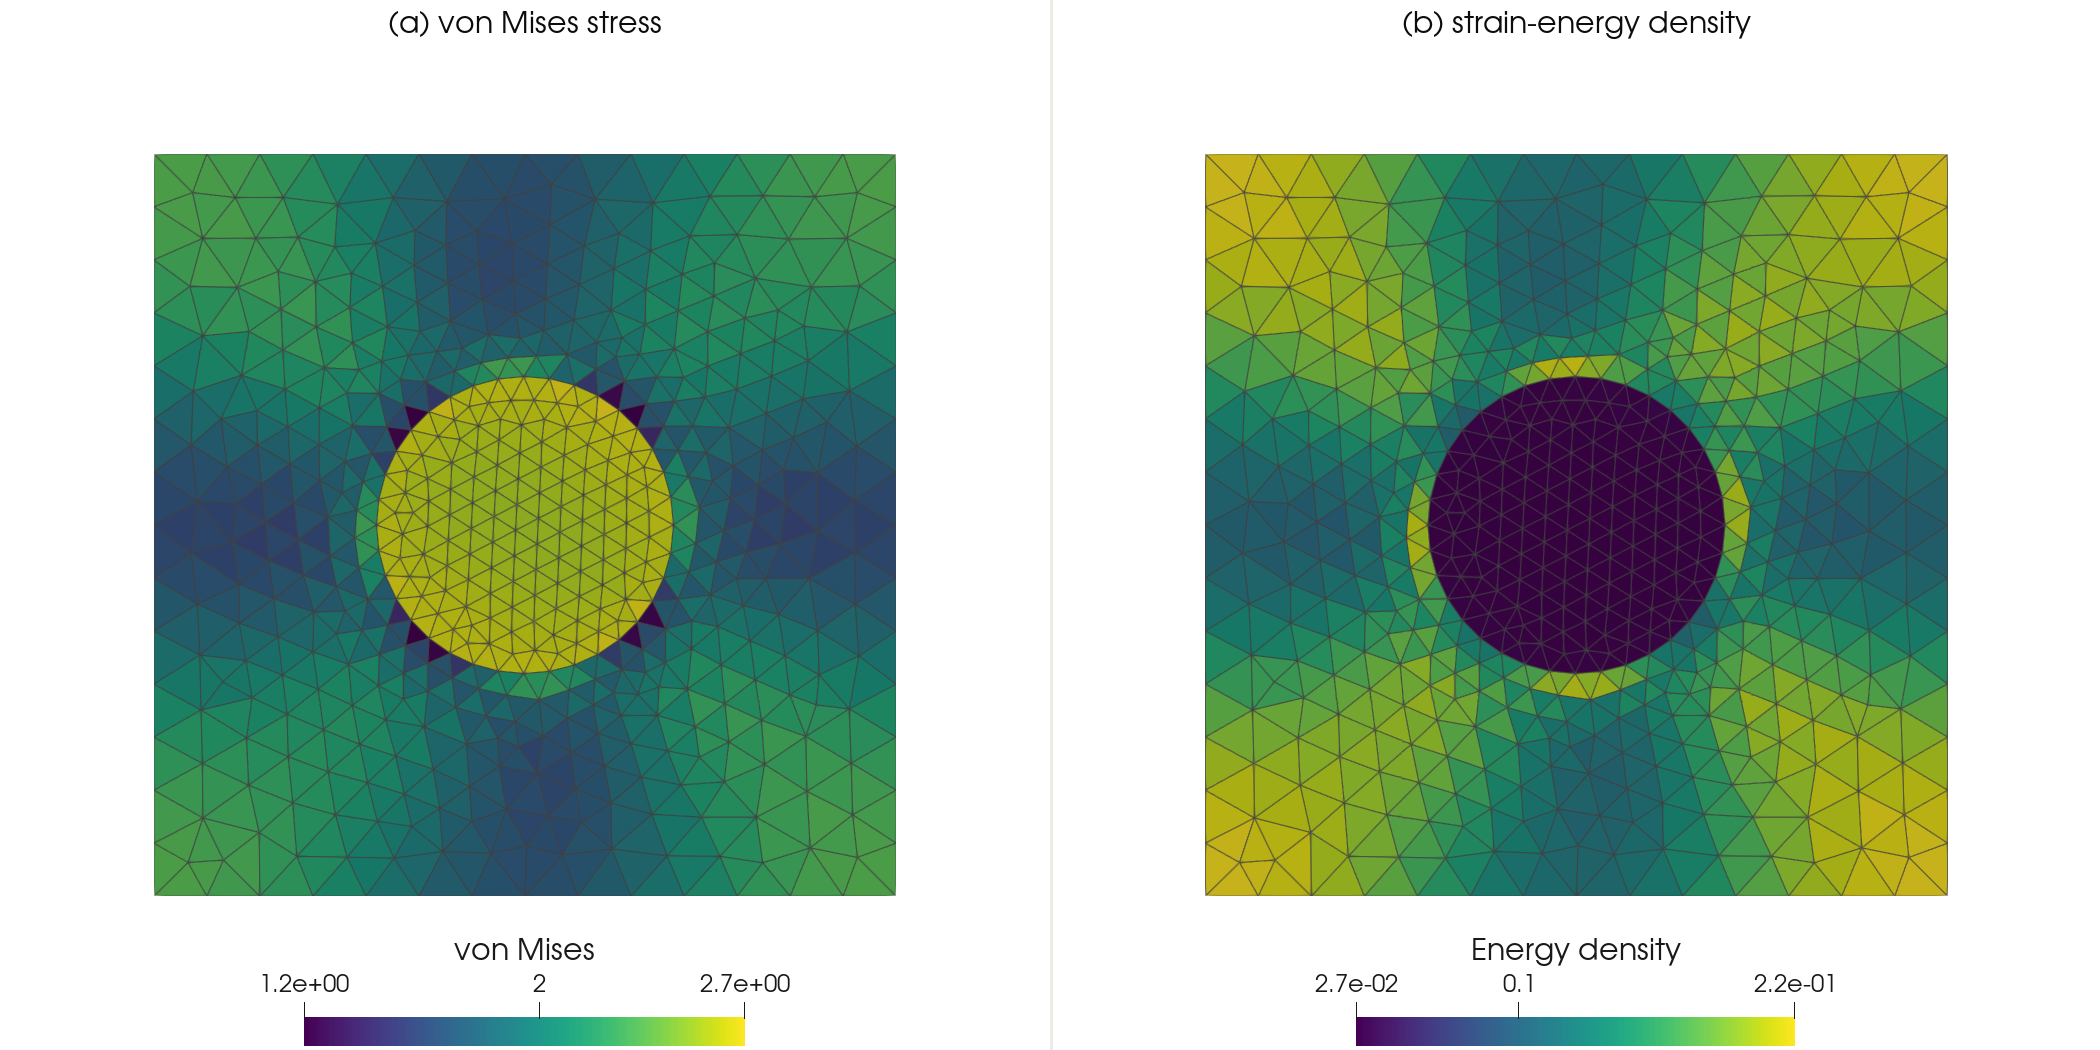
\includegraphics[width=\linewidth]{paraview_fields.png}
  \caption{ParaView rendering of the final state at engineering shear
  $\gamma_{12}=0.25$ for a two-phase Neo-Hookean cell. (a) von Mises stress;
  (b) strain-energy density. The field data are exported by HomiCSx and mesh
  edges are retained to distinguish the numerical field from a schematic.}
  \label{fig:fields}
\end{figure}

\subsection{Representative execution cost}

For scale rather than as a performance benchmark, examples were run on one
rank under WSL2 with Python 3.10.21 and DOLFINx 0.9.0 on an AMD Ryzen 9 9900X.
OMP, OpenBLAS, and MKL thread counts were fixed to one. After one untimed
warm-up, three independent process launches were measured with GNU
\texttt{/usr/bin/time -f ``\%e \%M'' conda run -n homicsx\_dev python
<script>}. The 2D linear case (264 triangles; 298 unconstrained displacement
DOFs; three load cases) took 1.80--1.83~s and 241~MiB peak RSS. The 3D linear
case (1441 tetrahedra; 1206 DOFs; six load cases) took 2.16~s and 252--259~MiB.
The 2D hyperelastic case (264 triangles; 298 DOFs; two increments) took
1.81--1.82~s and 241~MiB, and the three-increment viscoelastic case on the same
mesh took 1.89--2.03~s and 243~MiB. Times include Conda process startup. These
compact examples are workflow checks, not mesh-converged production
benchmarks, and no parallel speedup is claimed.

\section{Verification and validation}

The automated test suite covers deterministic geometry behavior, tagging,
periodic mesh construction, public API behavior, hook semantics, constitutive
parameter validation, and solver integration. Homogeneous 2D plane-strain and
six-load-case 3D linear problems are compared with analytical isotropic
stiffness. A deterministic 2D refinement gate reduces relative stiffness error
from 2.543\% on the coarse mesh to 0.211\% on the refined mesh. Neo-Hookean
first Piola stress is independently checked against numerical energy
derivatives in 2D and 3D, and an end-to-end nonlinear patch recovers analytical
macroscopic energy, stress, and mean Jacobian.

Because periodic-boundary enforcement is a consequential implementation choice
in multiscale homogenization \cite{henys2019}, the external validation suite
includes a boundary-split geometry. It uses independently generated Abaqus
models and only conventional macroscopic quantities. Three linear plane-strain
cases---a homogeneous non-unit cell, a centered 20\% circular inclusion, and a
periodic boundary-split inclusion---have maximum stiffness, probe-stress, and
probe-energy differences below 0.55\%. Homogeneous finite simple shear agrees
to within 0.00016\% for macro energy and shear stress. The automated canonical
gate regenerates both linear and homogeneous nonlinear HomiCSx results from
the current checkout before comparison with the archived Abaqus reference.

Generalized-Maxwell validation compares complete macro-shear-stress relaxation
histories. The homogeneous 2D and 3D curves agree with Abaqus to within
0.00063\% and 0.00068\% peak-normalized maximum error, respectively. For a
viscoelastic matrix containing a hyperelastic inclusion, the centered and
periodic-split 2D cases give 1.22\% and 1.35\% maximum curve errors. Automated
fast/slow-rate regressions in 2D and 3D additionally require different
converged heterogeneous fluctuation fields. The viscoelastic external curves
are paired archived datasets; current-code regression is supplied by the
analytical and heterogeneous rate tests rather than by rerunning Abaqus in CI.
The external evidence does not
establish pointwise field identity, all loading paths, or external validation
of a heterogeneous 3D viscoelastic cell. Figure~\ref{fig:visco-validation}
shows the complete relaxation histories used for the viscoelastic comparisons
rather than only their scalar error summaries.

\begin{figure}[htbp]
  \centering
  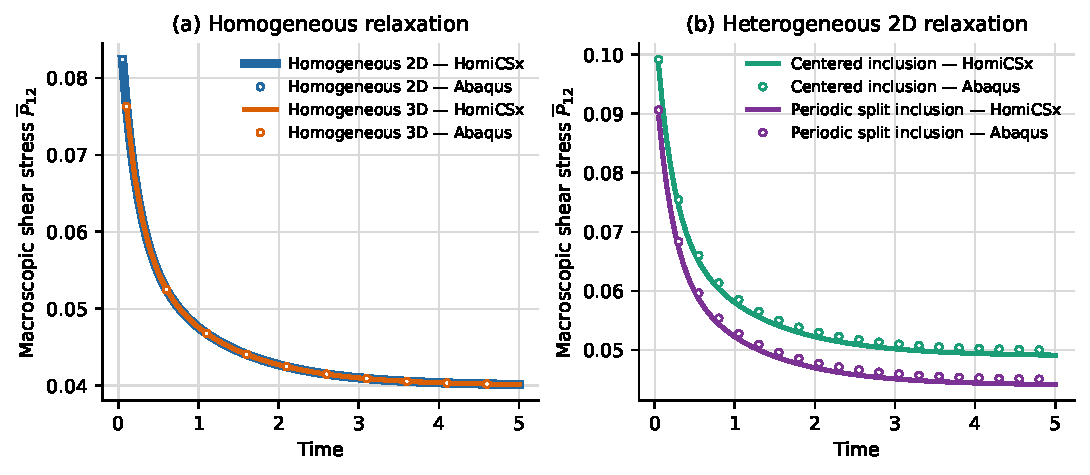
\includegraphics[width=\linewidth]{viscoelastic_validation.pdf}
  \caption{HomiCSx and Abaqus generalized-Maxwell shear-relaxation histories.
  Solid lines denote HomiCSx and open markers denote Abaqus. (a) Homogeneous 2D
  and 3D cells; (b) centered and periodic-split hyperelastic inclusions in a
  viscoelastic matrix.}
  \label{fig:visco-validation}
\end{figure}

\section{Impact and reuse}

HomiCSx enables a researcher to move from a seeded particulate description to
homogenized linear, hyperelastic, or viscoelastic response in one inspectable
workflow. Its hook mechanism is particularly relevant when a study needs
quantities or interventions that are not general enough to belong in a fixed
post-processing interface. The software is already used by its author in a
study of matrix localization in random periodic composites; that application
uses custom material and field-processing logic while retaining the common
geometry, mesh, equilibrium, and homogenization pipeline.

Potential reuse includes parametric studies of particulate composites,
development and comparison of constitutive laws, generation of training data
for reduced-order or surrogate models, and teaching reproducible RVE analysis.
No claim of external adoption is made at this stage. The MIT license, public
interfaces, tests, and archived releases are intended to allow independent use
and continuation.

\section{Limitations and maintenance}

The tested environment is Linux, including Linux under WSL2, with Python 3.10,
DOLFINx 0.9.0, and dolfinx\_mpc 0.9.0. Two-dimensional FEM uses plane strain;
plane stress is not implemented. The supported meshing path uses triangles,
tetrahedra, and tested 2D all-quadrilateral meshes, although viscoelastic state
updates require simplex cells; general 3D hexahedral meshing is not
implemented. Imported meshes, independently oriented random
nonspherical packing, overlapping-void and open-cell workflows,
advanced visualization, and stochastic convenience modules are outside the
publication-supported core. The latter two modules are explicitly
experimental.

HomiCSx is maintained as archival research software. No feature schedule or
guaranteed support response is promised. Reproducibility, documentation,
correctness fixes as resources permit, versioned releases, and preservation
are prioritized. The permissive license allows community forks and continued
development if active maintenance changes.

HomiCSx 1.x supports solver execution on one MPI rank. The drivers reject
distributed communicators until cross-rank consistency is established and
continuously tested.

\section{Conclusions}

HomiCSx provides a tested, inspectable path from periodic particulate geometry
to homogenized linear, hyperelastic, and generalized-Maxwell response. Its
principal value is integration with explicit research extension points rather
than a new homogenization theory. The release combines a bounded supported
core, conventional analytical and Abaqus evidence, reproducible environments,
and candid limitations. This makes the software suitable for customized RVE
studies while keeping its archival maintenance commitment realistic.

\section{Availability and reproducibility}

\begin{description}
  \item[Source code:] \url{https://github.com/AmirTahouni/HomiCSx}
  \item[Documentation:] \url{https://homicsx.readthedocs.io/en/latest/}
  \item[License:] MIT
  \item[Version described:] 1.0.1
  \item[Version archive:] \url{https://github.com/AmirTahouni/HomiCSx/tree/v1.0.1}
  \item[Concept DOI:] \url{https://doi.org/10.5281/zenodo.22811693}
\end{description}

The repository contains version-constrained Conda environment specifications, installation
instructions, automated tests, benchmark manifests, independently constructed
Abaqus model runners
scripts, compact reference results, and executable acceptance gates. Abaqus is
not required to recompute comparisons from the committed compact results.

\section*{CRediT authorship contribution statement}

\textbf{Amir Reza Tahouni:} Conceptualization, Methodology, Software,
Validation, Investigation, Data curation, Visualization, Writing---original
draft, Writing---review and editing.

\section*{Funding}

This research did not receive any specific grant from funding agencies in the
public, commercial, or not-for-profit sectors.

\section*{Declaration of competing interest}

The author declares no known competing financial interests or personal
relationships that could have appeared to influence the work reported in this
paper.

\section*{Data availability}

The software, validation manifests, scripts, and compact numerical results are
available in the public repository and are preserved in the archived release
identified above. Large proprietary Abaqus working databases are not
required to evaluate the committed comparison results and are not distributed.

\section*{Declaration of generative AI and AI-assisted technologies in the manuscript preparation process}

During the preparation of this work, the author used an OpenAI coding assistant
to support code review, test and validation development, documentation editing,
and manuscript drafting. After using this service, the author reviewed and
edited the content as needed and takes full responsibility for the content of
the publication.

\small
\begin{thebibliography}{00}

\bibitem{dolfinx2025}
I. A. Baratta, J. P. Dean, J. S. Dokken, et al., DOLFINx: The next generation
FEniCS problem solving environment, preprint (2025).
\url{https://doi.org/10.5281/zenodo.18101307}.

\bibitem{ufl2014}
M. S. Aln\ae s, A. Logg, K. B. \O lgaard, M. E. Rognes, G. N. Wells, Unified
Form Language: A domain-specific language for weak formulations of partial
differential equations, ACM Trans. Math. Softw. 40 (2) (2014) Article 9,
1--37.
\url{https://doi.org/10.1145/2566630}.

\bibitem{gmsh2009}
C. Geuzaine, J.-F. Remacle, Gmsh: A 3-D finite element mesh generator with
built-in pre- and post-processing facilities, Int. J. Numer. Methods Eng. 79
(11) (2009) 1309--1331. \url{https://doi.org/10.1002/nme.2579}.

\bibitem{geers2003}
M. G. D. Geers, V. G. Kouznetsova, W. A. M. Brekelmans, Multi-scale
first-order and second-order computational homogenization of microstructures
towards continua, Int. J. Multiscale Comput. Eng. 1 (4) (2003) 371--386.
\url{https://doi.org/10.1615/IntJMultCompEng.v1.i4.40}.

\bibitem{saeb2016}
S. Saeb, P. Steinmann, A. Javili, Aspects of computational homogenization at
finite deformations: A unifying review from Reuss' to Voigt's bound, Appl.
Mech. Rev. 68 (5) (2016) 050801.
\url{https://doi.org/10.1115/1.4034024}.

\bibitem{henys2019}
P. Heny\v{s}, L. \v{C}apek, J. B\v{r}ezina, Comparison of current methods for
implementing periodic boundary conditions in multi-scale homogenisation, Eur.
J. Mech. A Solids 78 (2019) 103825.
\url{https://doi.org/10.1016/j.euromechsol.2019.103825}.

\bibitem{homicsx2026}
A. R. Tahouni, HomiCSx, version 1.0.1, GitHub (2026).
\url{https://github.com/AmirTahouni/HomiCSx/tree/v1.0.1}.

\bibitem{microstructpy2020}
K. A. Hart, J. J. Rimoli, MicroStructPy: A statistical microstructure mesh
generator in Python, SoftwareX 12 (2020) 100595.
\url{https://doi.org/10.1016/j.softx.2020.100595}.

\bibitem{damask2020}
M. Diehl, D. Wang, C. Liu, et al., Solving material mechanics and multiphysics
problems of metals with complex microstructures using DAMASK, Adv. Eng. Mater.
22 (2020) 1901044. \url{https://doi.org/10.1002/adem.201901044}.

\bibitem{moose2020}
C. J. Permann, D. R. Gaston, D. Andr\v{s}, et al., MOOSE: Enabling massively
parallel multiphysics simulation, SoftwareX 11 (2020) 100430.
\url{https://doi.org/10.1016/j.softx.2020.100430}.

\bibitem{micmacsfenics}
F. Rocha, micmacsfenics: a FEniCS-based implementation of two-level finite
element simulations using computational homogenization, software repository
(accessed 18 September 2026).
\url{https://github.com/felipefr/micmacsfenics}.

\bibitem{fenicshomogenization}
B. Shrimali, FEniCS\_homogenization: a collection of homogenization scripts for
linear elasticity, software repository (accessed 18 September 2026).
\url{https://github.com/bhaveshshrimali/FEniCS_homogenization}.

\end{thebibliography}

\end{document}
